\Chapter{Tesztek, eredmények}

% TODO: Be kell mutatni, hogy milyen módon került validálásra az elkészült eszköz!
% TODO: Itt lehet akár egy kisebb felhasználói kézikönyv félét is betenni!
% TODO: Minden lényeges funkcióhoz jó lenne, ha szerepelne majd képernyőkép!

Mivel a program Rust nyelvben íródott, és a program mivolta egy Rust fejlesztői környezet,
így a legegyszerűbb módja a program tesztelésének a program kódjának megvizsgálása saját magán belül.

\Section{Fájlkezelés}

\begin{wrapfigure}{r}{0.4\textwidth}
    \centering
    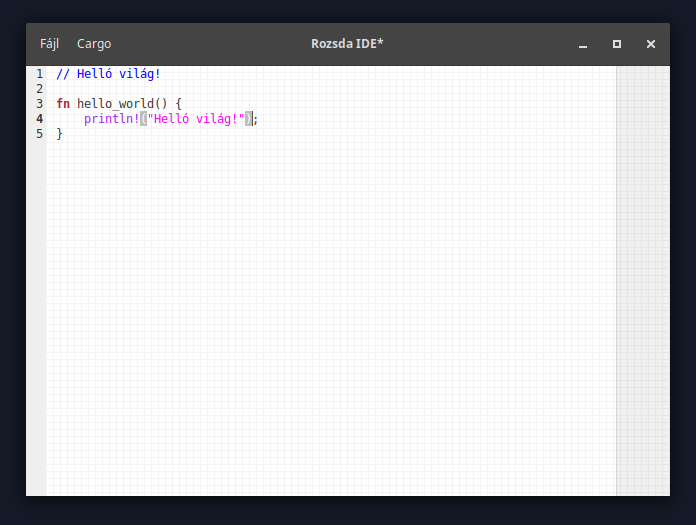
\includegraphics[width=0.4\textwidth]{nevtelen-fajl}
\end{wrapfigure}

A fájlkezelési műveletek teszteléséhez létrehozunk egy fájlt, ami egyetlen metódust tartalmaz,
és kiíratja, hogy "Helló világ!". 
Láthatjuk, hogy ahogy a pufferbe szöveget viszünk be, a program címéhez hozzá kerül egy "*",
jelezve, hogy a puffer eltér a várttól -- ebben az esetben nincs fájl a háttértáron,
így amíg van valami a pufferben, az mindig mentetlen módosításnak számít.

A megírt metódust megfogjuk hívni a Rozsda IDE-n belül, így a fájlt elmentjük \texttt{hello.rs}
néven a Rozsda IDE ládájába.

\begin{wrapfigure}{l}{0.35\textwidth}
    \centering
    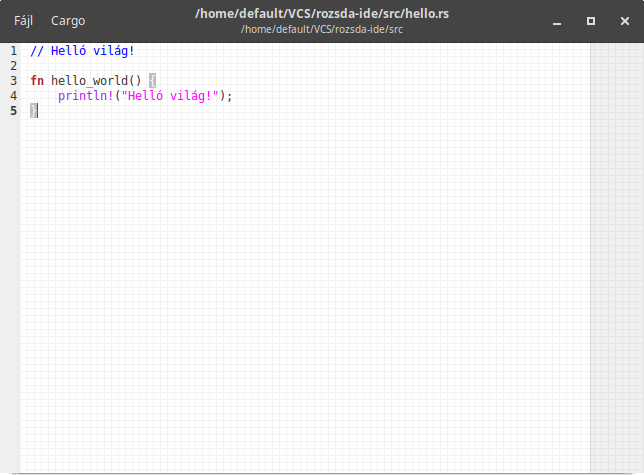
\includegraphics[width=0.35\textwidth]{elmentett-fajl}
    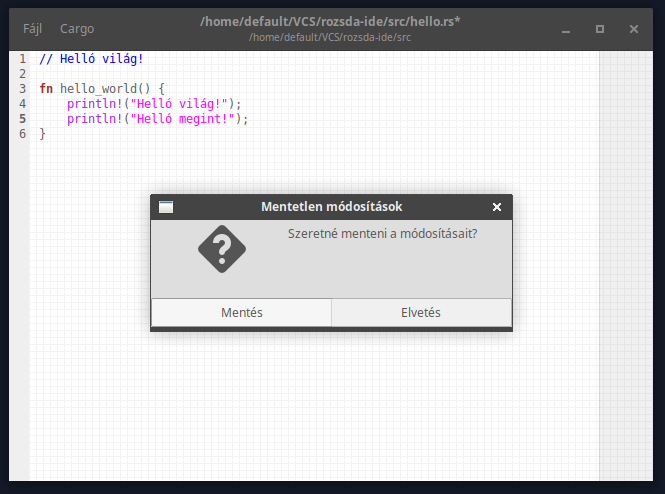
\includegraphics[width=0.35\textwidth]{kilepes-mentetlen-valtozasokkal}
\end{wrapfigure}

Itt mind a \texttt{Ctrl+S} billentyűkombináció, mind a \textit{Fájl $\,\to\,$ Mentés} vagy \textit{Fájl $\,\to\,$ Mentés Másként}
lehetőségek sikeresen elmentik a fájlt a felhasználó által kiválasztott helyre.
A mentés után a program címe a szerkesztett fájl elérési útvonalára változik,
míg alcímnek az azt tartalmazó könyvtár kerül.
Ha ezek után tovább szerkesztjük a fájlt, akkor megint észrevehetjük,
hogy a szerkesztéssel a cím egy "*" jelet kap, ha a tartalom eltér a háttértáron lévő fájl tartalmától.
Ha nem mentjük a változtatásainkat, 
hanem inkább bezárjuk a fájlt a \textit{Fájl $\,\to\,$ Bezárás} menüelemmel vagy a \texttt{Ctrl+W} billentyűkombinációval,
vagy bezárjuk az egész programot a \textit{Fájl $\,\to\,$ Kilépés} elemmel vagy a \texttt{Ctrl+Q} billentyűkombinációval,
akkor a program figyelmeztet, hogy mentetlen változtatásaink vannak,
és felajánlja, hogy azokat mentsük, vagy elvessük.

Az előbbi lehetőség választása esetén megtörténik a mentés,
az utóbbi esetén viszont a program kiüríti a belső pufferét, és elfelejti a háttértári fájl elérési útvonalát.
Mindkét döntés esetében megtörténik a kívánt művelet (bezárás vagy kilépés) a módosítások lekezelése után.

\Section{Projektkezelés}

\begin{wrapfigure}{l}{0.4\textwidth}
    \centering
    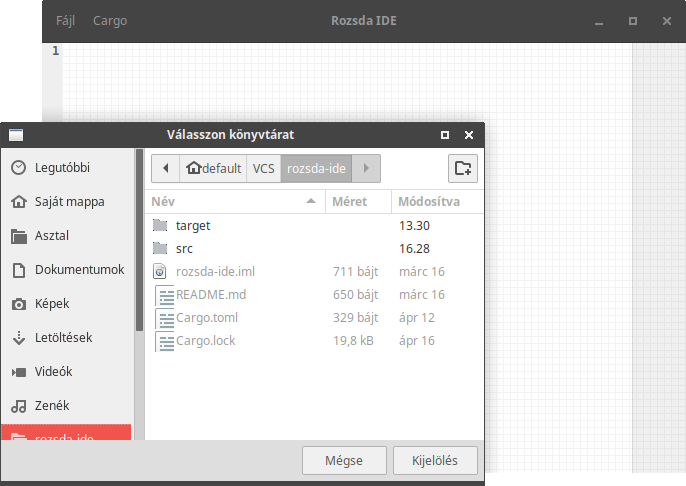
\includegraphics[width=0.4\textwidth]{projekt-megnyitas}
\end{wrapfigure}

Ha a \textit{Cargo $\,\to\,$ Megnyitás} lehetőséget választjuk, akkor A program felajánlja
nekünk egy tetszőleges könyvtár kiválasztását a háttértárainkon.
Itt tetszőlegesen navigálhatunk, illetve, ha szükséges, létrehozhatunk új könyvtárakat is.

Ha egy olyan könyvtárat választottunk, ami tartalmaz egy \texttt{Cargo.toml} fájlt,
akkor a projektmegnyitás sikeresen betölti a ládát.
Fontos nem elfelejteni, hogy ilyenkor új fájl nem töltődik be,
így még mindig a legutóbb megnyitott fájlt fogjuk látni a módosításainkkal, ha vannak.

Sikeres projektmegnyitás esetén a láda főkönyvtárának neve beillesztődik a program címébe,
a fájl (vagy a Rozsda IDE) neve után, egy kötőjellel elválasztva attól.

Ha olyan könyvtárat választunk ki, ami nem tartalmaz egy \texttt{Cargo.toml} fájlt,
akkor egy felugró ablak értesít minket arról, hogy a megnyitni kívánt projekt nem
érvényes Rust láda.
A felugró ablakot elfogadva bezáródik mind az, mind a könyvtárválasztó ablak.

Mint a sikeres projektmegnyitás, a megnyitott fájlunkra ez sincs kihatással.

\begin{figure}[h]
    \centering
    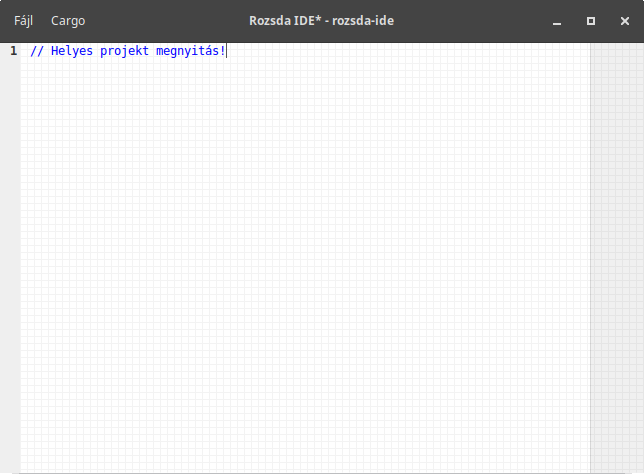
\includegraphics[width=0.4\textwidth]{projekt-megnyitas-sikeres}
    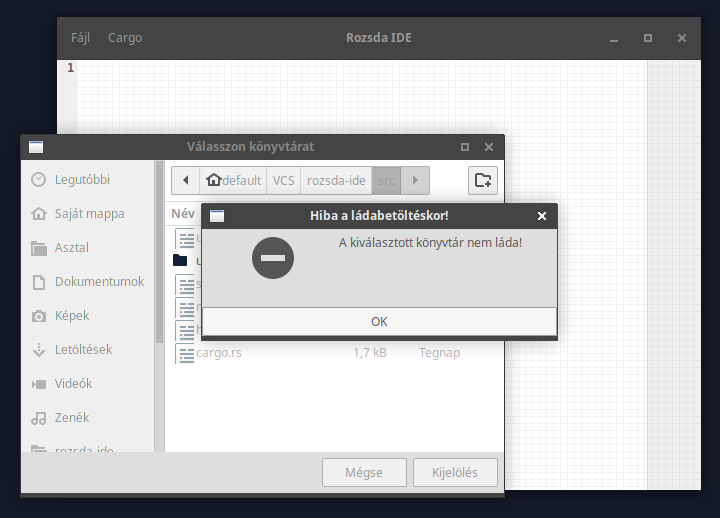
\includegraphics[width=0.4\textwidth]{projekt-megnyitas-sikertelen}
\end{figure}

Ha a \textit{Cargo $\,\to\,$ Új könyvtár} vagy a \textit{Cargo $\,\to\,$ Új bináris}
lehetőségeket választjuk ki, akkor a program felajánlja nekünk,
hogy kiválasszunk illetve készítsünk egy új (fájlrendszeri) könyvtárat,
amibe aztán előkészíti nekünk a könyvtár vagy bináris láda alapvető elemeit.

Az újonnan létrehozott láda tartalmát megvizsgálva az előbbi esetben egy \texttt{lib.rs}
fájlt fogunk találni az \texttt{src/} könyvtárban, ami el van látva egy példa teszttel, 
az utóbbi esetben egy \texttt{main.rs} fájlt, amiben egy alapvető \texttt{main()} metódus található.

\begin{figure}[h]
    \centering
    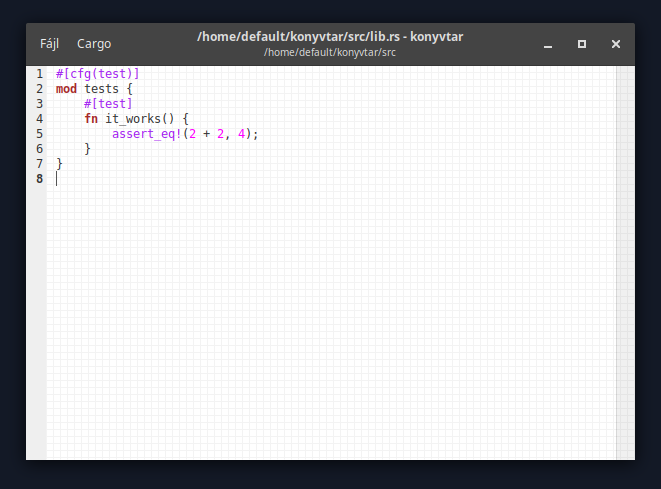
\includegraphics[width=0.4\textwidth]{uj-konyvtar}
    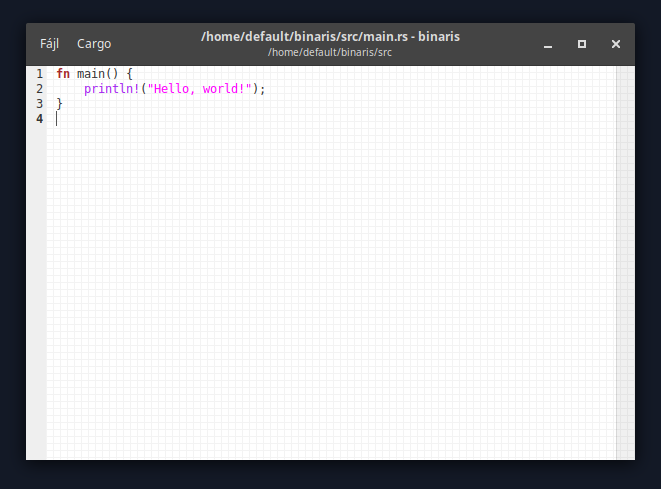
\includegraphics[width=0.4\textwidth]{uj-binaris}
\end{figure}

\newpage

\Section{Cargo parancsok}

\begin{wrapfigure}{l}{0.30\textwidth}
    \centering
    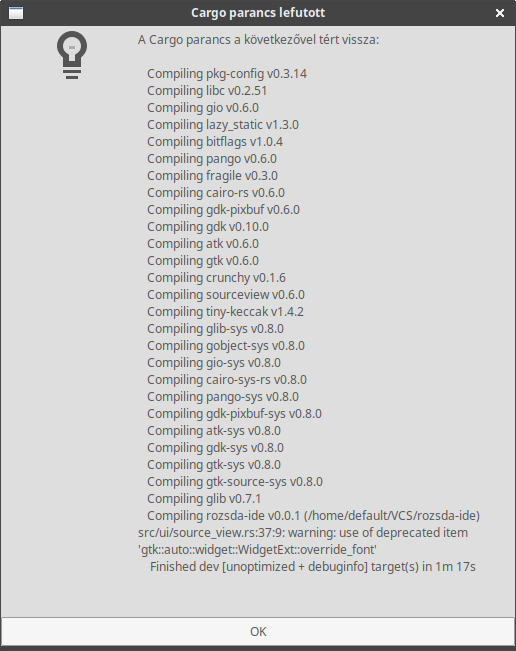
\includegraphics[width=0.30\textwidth]{forditas}
\end{wrapfigure}

A Rozsda IDE ládájának megnyitása után kipróbálhatjuk a Cargo parancsokat.
Mivel ahhoz, hogy a Rozsda IDE-t futtassam, le kellett fordítanom,
így először a \textit{Cargo $\,\to\,$ Takarítás} lehetőséget tesztelem le.

Bár egy felugró ablak megjelenik, a \texttt{cargo clean} parancs nem ad kimenetet,
így csak egy felugró ablakot kapunk, ami értesít minket a parancs lefutásáról.

Ezek után, ha módosítjuk a \texttt{main.rs}-t, hogy hívja meg az újonnan készített
\texttt{hello.rs} fájlunkból a \texttt{hello\_world()} metódust,
lefordíthatjuk a ládát a \textit{Cargo $\,\to\,$ Fordítás} lehetőséggel.

Fordítani külön nem szükséges.
Ha a \textit{Cargo $\,\to\,$ Futtatás} lehetőséget választottuk volna,
a ládának ugyanúgy le kell fordulnia, viszont a teljes tesztelés érdekében
először fordítunk, majd utána futtatjuk a programot.

A legtöbb parancs, ami szükségelteti a program lefordulását (mint az \textit{Ellenőrzés,}
vagy a \textit{Tesztek futtatása}), ugyanúgy meghívja a \texttt{cargo build} parancsot.

A program lefordulásával kapunk egy listát az összes lefordult könyvtárról és bináris ládáról,
az összes figyelmeztetésről és hibáról, illetve, hogy ha lefordítás sikeres,
akkor a fordítás idejéről is.

\begin{figure}[h]
    \centering
    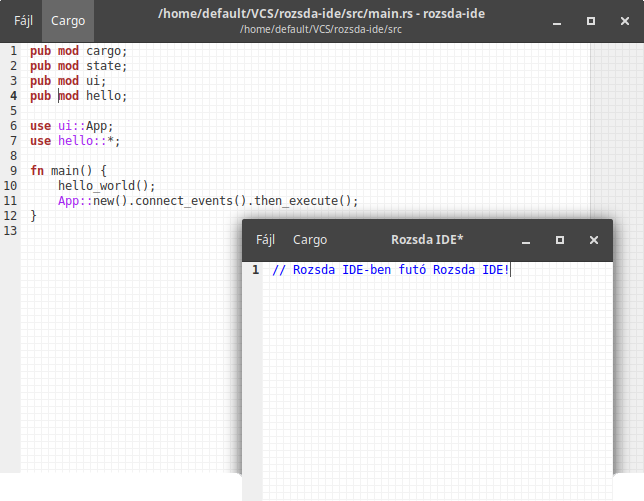
\includegraphics[width=0.4\textwidth]{rozsda-ide-rozsda-ideben}
    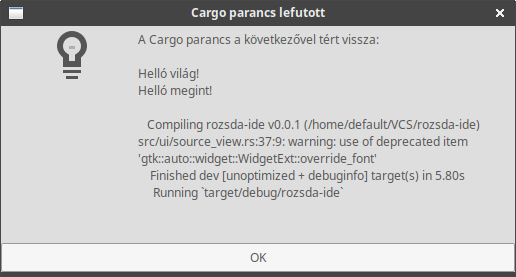
\includegraphics[width=0.4\textwidth]{rozsda-ide-visszateres}
\end{figure}

A program lefordulásával futtathatjuk is a ládánkat.
A jobbra látható képen elindítottam a Rozsda IDE-t a Rozsda IDE-ben.
A program működése megegyezik az őt fordító és futtató programéval, bár kettő
\texttt{println!}-nel több parancs van benne.

Ezeket a kiíratásokat a program befejeztetése után megkapjuk.
